% Basic Category Theory
% Tom Leinster <Tom.Leinster@ed.ac.uk>
% 
% Copyright (c) Tom Leinster 2014-2016
% 
% Chapter 3: Interlude on sets
% 

\chapter{Interlude on sets}
\label{ch:sets}

Sets and functions are ubiquitous in mathematics.  You might have the
impression that they are most strongly connected with the pure end of the
subject, but this is an illusion: think of probability density functions in
statistics, data sets in experimental science, planetary motion in
astronomy, or flow in fluid dynamics.

Category theory is often used to shed light on common constructions and
patterns in mathematics.  If we hope to do this in an advanced context, we
must begin by settling the basic notions of set and function.  That is the
purpose of the first section of this chapter.

The definition of category mentions a `collection' of objects and
`collections' of maps.  We will see in the second section that some
collections are too big to be sets, which leads to a distinction between
`small' and `large' collections.  This distinction will be needed later,
most prominently for the adjoint functor theorems (Chapter~\ref{ch:arl}).

The final section takes a historical look at set theory.  It also explains
why the approach to sets taken in this chapter is more relevant to most of
mathematics than the traditional approach is.  None of this section is
logically necessary for anything that follows, but it may provide useful
perspective.

I do not assume that you have encountered axiomatic set theory of any kind.
If you have, it is probably best to put it out of your mind while reading
this chapter, as the approach to set theory that we take is quite different
from the approach that you are most likely to be familiar with.  A brief
comparison of the traditional and categorical approaches can be found at
the very end of the chapter.



\section{Constructions with sets}
\label{sec:Set-properties}


We have made no definition of `set', nor of `function'.  Nevertheless,
guided by our intuition, we can list some properties that we expect the
world of sets and functions to have.  For instance, we can describe some
of the sets that we think ought to exist, and some ways of building new
sets from old.

Intuitively,%
%
\index{set!intuitive description of}
%
a set is a bag of points:
\[
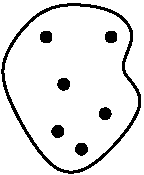
\includegraphics[height=5em]{set}
\]
(There may, of course, be infinitely many.)  These points, or elements, are
not%
%
\index{set!structurelessness of}
%
related to one another in any way.  They are not in any order, they do not
come with any algebraic structure (for instance, there is no specified way
of multiplying elements together), and there is no sense of what it means
for one point to be close to another.  In particular examples, we might
have some extra structure in mind; for instance, we often equip the set of
real numbers with an order, a field structure and a metric.  But to view
$\reals$ as a mere \emph{set} is to ignore all that structure, to regard it
as no more than a bunch of featureless points.

Intuitively,%
%
\index{function!intuitive description of}
%
a function $A \to B$ is an assignment of a point in bag $B$ to each point
in bag $A$:
\[
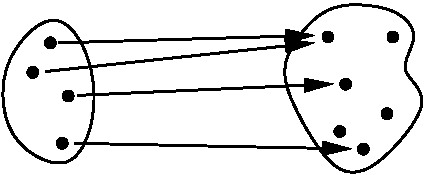
\includegraphics[height=5em]{function}
\]
We can do one function after another: given functions
\[
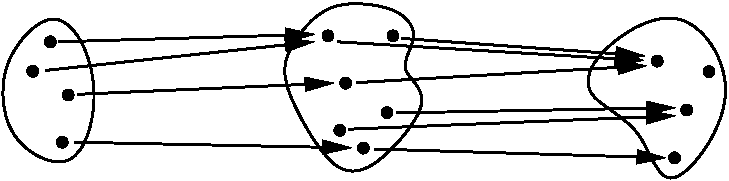
\includegraphics[height=5em]{composable}
\]
we obtain a composite function
\[
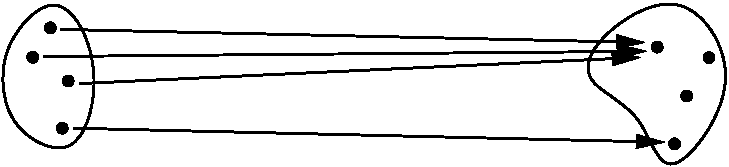
\includegraphics[height=4.6em]{composed}
\]
This composition of functions is associative: $h \of (g \of f) =
(h \of g) \of f$.  There is also an identity function on every set.  Hence:
% 
\begin{setprop}
Sets and functions form a category, denoted by $\Set$.%
%
\index{set!category of sets}
%
\end{setprop}

This does not pin things down much: there are many categories, mostly quite
unlike the category of sets.  So, let us list some of the special features
of the category of sets.

\paragraph*{The empty set}  
%
\index{set!empty}
%
There is a set $\emptyset$ with no elements.

Suppose that someone hands you a pair of sets, $A$ and $B$, and tells you
to specify a function from $A$ to $B$.  Then your task is to specify for
each element of $A$ an element of $B$.  The larger $A$ is, the longer the
task; the smaller $A$ is, the shorter the task.  In particular, if $A$ is
empty then the task takes no time at all; we have nothing to do.  So there
is a function from $\emptyset$ to $B$ specified by doing nothing.  On the
other hand, there cannot be two different ways to do nothing, so there is
only one function from $\emptyset$ to $B$.  Hence:
% 
\begin{setprop}
$\emptyset$ is an initial object of \hspace{.1em}$\Set$.
\end{setprop}

In case this argument seems unconvincing, here is an alternative.  Suppose
that we have a set $A$ with disjoint subsets $A_1$ and $A_2$ such that $A_1
\cup A_2 = A$.  Then a function from $A$ to $B$ amounts to a function from
$A_1$ to $B$ together with a function from $A_2$ to $B$.  So if all the
sets are finite, we should have the rule
% 
\begin{align*}  
\label{p:num-fns}
%
\index{function!number of functions}
%
(\text{number of functions from $A$ to $B$})	&
=	
(\text{number of functions from $A_1$ to $B$})	\\
& \quad\times
(\text{number of functions from $A_2$ to $B$}).
\end{align*}
% 
In particular, we could take $A_1 = A$ and $A_2 = \emptyset$.  This would
force the number of functions from $\emptyset$ to $B$ to be $1$.  So if we
want this rule to hold (and surely we do!), we had better say that there is
exactly one function from $\emptyset$ to $B$.

What about functions \emph{into} $\emptyset$?  There is exactly one function
$\emptyset \to \emptyset$, namely, the identity.  This is a special case of
the initiality of $\emptyset$.  On the other hand, for a set $A$ that is not
empty, there are no functions $A \to \emptyset$, because there is nowhere for
elements of $A$ to go.


\paragraph*{The one-element set}  
%
\index{set!one-element}
%
There is a set $1$ with exactly one element.

For any set $A$, there is exactly one function from $A$ to $1$, since every
element of $A$ must be mapped to the unique element of $1$.  That is:
% 
\begin{setprop}
$1$ is a terminal object of \hspace{.1em}$\Set$.
\end{setprop}

A function \emph{from} $1$ \emph{to} a set $B$ is just a choice of an element
of $B$.  In short, the functions $1 \to B$ are the elements of $B$.  Hence:
% 
\begin{slogan}
The concept of element is a special case of the concept of function.%
%
\index{element!function@as function}
%
\end{slogan} 

\paragraph*{Products}  Any two sets $A$ and $B$ have a product,%
%
\index{set!category of sets!products in}
%
$A \times B$.%
%
\ntn{prod-set}
%
  Its elements are the ordered pairs $(a, b)$ with $a \in A$
and $b \in B$.  Ordered pairs are familiar from coordinate geometry.  All
that matters about them is that for $a, a' \in A$ and $b, b' \in B$,
\[
(a, b) = (a', b')
\iff
a = a' \text{ and } b = b'.
\]
More generally, take any set $I$ and any family $(A_i)_{i \in I}$ of sets.
There is a product set $\prod_{i \in I} A_i$,%
%
\ntn{prod-fam-set}
%
whose elements are families%
%
\index{family}
%
$(a_i)_{i \in I}$ with $a_i \in A_i$ for each $i$.  Just as for ordered
pairs,
\[
(a_i)_{i \in I} = (a'_i)_{i \in I}
\iff
a_i = a'_i \text{ for all } i \in I.
\]

\paragraph*{Sums}  Any two sets $A$ and $B$ have a \demph{sum}%
%
\index{set!category of sets!sums in}
%
$A + B$.%
%
\ntn{sum-set}
%


Thinking of sets as bags of points, the sum of two sets is obtained by
putting all the points into one big bag:
\[
\begin{array}{c}
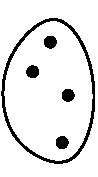
\includegraphics[height=5em]{sumL}
\end{array}
\, + \,
\begin{array}{c}
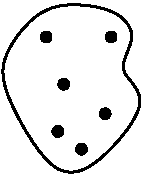
\includegraphics[height=5em]{sumR}
\end{array}
\ = \
\begin{array}{c}
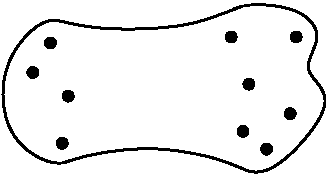
\includegraphics[height=5em]{sumtot}
\end{array}
\]
If $A$ and $B$ are finite sets with $m$ and $n$ elements respectively, then
$A + B$ always has $m + n$ elements.  It makes no difference what the
elements of $A + B$ are called; as usual, we only care what $A + B$ is up
to isomorphism.

There are inclusion functions
\[
A \toby{i} A + B \otby{j} B
\]
such that the union of the images of $i$ and $j$ is all of $A + B$ and the
intersection of the images is empty.

Sum is sometimes called \demph{disjoint union}%
%
\index{disjoint union}
%
and written as $\amalg$.%
%
\ntn{disjt-union}
%
It is not to be confused with (ordinary) union%
%
\index{union}
%
$\cup$.  For a start, we can take the sum of \emph{any} two sets $A$ and
$B$, whereas $A \cup B$ only really makes sense when $A$ and $B$ come as
subsets of some larger set.  (For to say what $A \cup B$ is, we need to
know which elements of $A$ are equal to which elements of $B$.)  And even
if $A$ and $B$ do come as subsets of some larger set, $A + B$ and $A \cup
B$ can be different.  For example, take the subsets $A = \{1, 2, 3\}$ and
$B = \{3, 4\}$ of $\nat$.  Then $A \cup B$ has $4$ elements, but $A + B$
has $3 + 2 = 5$ elements.
  
More generally, any family $(A_i)_{i \in I}$ of sets has a sum $\sum_{i \in
I} A_i$.%
%
\ntn{sum-fam-set}
%
If $I$ is finite and each $A_i$ is finite, say with $m_i$
elements, then $\sum_{i \in I} A_i$ has $\sum_{i \in I} m_i$ elements.

\paragraph*{Sets of functions}  
%
\index{set!functions@of functions}%
\index{function!set of functions}
%
For any two sets $A$ and $B$, we can form the set $A^B$%
%
\ntn{exponential-set}
%
 of functions from $B$ to $A$.  

This is a special case of the product construction: $A^B$ is the product
$\prod_{b \in B} A$ of the constant family $(A)_{b \in B}$.  Indeed, an
element of $\prod_{b \in B} A$ is a family $(a_b)_{b \in B}$ consisting of
one element $a_b \in A$ for each $b \in B$; in other words, it is a function
$B \to A$.

\paragraph*{Digression on arithmetic}%  
\label{p:arith}
%
\index{arithmetic}
% 
We are using notation reminiscent of arithmetic: $A \times B$, $A + B$, and
$A^B$.  There is good reason for this: if $A$ is a finite set with $m$
elements and $B$ a finite set with $n$ elements, then $A \times B$ has $m
\times n$ elements, $A + B$ has $m + n$ elements, and $A^B$ has $m^n$
elements.  Our notation $1$ for a one-element set and the alternative
notation $0$ for the empty set $\emptyset$ also follow this pattern.

All the usual laws of arithmetic have their counterparts for sets:
% 
\begin{align*}
A \times (B + C)        &\iso (A \times B) + (A \times C),      \\
A^{B + C}               &\iso A^B \times A^C,                   \\
(A^B)^C                 &\iso A^{B \times C},
\end{align*}
% 
and so on, where $\iso$ is isomorphism in the category of sets.  (For the
last one, see Example~\ref{eg:adjn:cc}.)  These isomorphisms hold for all
sets, not just finite ones.

\paragraph*{The two-element set}  
%
\index{set!two-element}
%
Let $2$%
%
\ntn{two-set}
%
be the set $1 + 1$ (a set with two elements!).  For reasons that will soon
become clear, I will write the elements of $2$ as $\true$ and $\false$.

Let $A$ be a set.  Given a subset%
%
\index{subset}
%
$S$ of $A$, we obtain a function $\chi_S\from A \to 2$%
%
\ntn{char-fn}
%
(the \demph{characteristic%
%
\index{characteristic function}%
\index{function!characteristic}
%
function} of $S \sub A$), where
\[
\chi_S(a)
=
\begin{cases}
\true	&\text{if }a \in S,	\\
\false	&\text{if }a \not\in S
\end{cases}
\]
($a \in A$).  Conversely, given a function $f\from A \to 2$, we obtain a
subset
\[
f^{-1}\{\true\} 
= 
\{ a \in A \such f(a) = \true \}
\]
of $A$.  These two processes are mutually inverse; that is, $\chi_S$ is the
unique function $f\from A \to 2$ such that $f^{-1}\{\true\} = S$.  Hence:
% 
\begin{setprop}
Subsets of $A$ correspond one-to-one with functions $A \to 2$.
\end{setprop}
% 
We already know that the functions from $A$ to $2$ form a set, $2^A$.  When we
are thinking of $2^A$ as the set of all subsets of $A$, we call it the
\demph{power%
%
\index{power!set}
%
set} of $A$ and write it as $\pset(A)$.%
%
\ntn{power-set-precise}
%


\paragraph*{Equalizers}  
%
\index{equalizer!sets@of sets}%
\index{set!category of sets!equalizers in}
% 
It would be nice if, given a set $A$, we could define a subset $S$ of $A$
by specifying a property that the elements of $S$ are to satisfy:
\[
S
=
\{ a \in A \such \text{some property of } a \text{ holds} \}.
\]
It is hard to give a general definition of `property'.  There is, however, a
special type of property that is easy to handle: equality of two functions.
Precisely, given sets and functions $\parpair{A}{B}{f}{g}$, there is a set
\[
\{ a \in A \such f(a) = g(a) \}.
\]
This set is called the \demph{equalizer} of $f$ and $g$, since it is the
part of $A$ on which the two functions are equal.

\paragraph*{Quotients}
You are probably familiar with quotient groups and quotient rings
(sometimes called factor groups and factor rings) in algebra.  Quotients
also come up everywhere in topology, such as when we glue together opposite
sides of a square to make a cylinder.  But the most basic context for
quotients is that of sets.

Let $A$ be a set and $\sim$ an equivalence%
%
\index{equivalence relation}
%
relation on $A$.  There is a set $\qer{A}{\sim}$,%
%
\ntn{qt-set}
%
the \demph{quotient of $A$ by $\sim$},%
%
\index{quotient!set@of set}%
\index{set!quotient of}
%   
whose elements are the equivalence classes.  For example, given a group $G$
and a normal subgroup $N$, define an equivalence relation $\sim$ on $G$ by
$g \sim h \iff gh^{-1} \in N$; then $\qer{G}{\sim} = G/N$.

There is also a canonical map
\[
p\from A \to \qer{A}{\sim},
\]
sending an element of $A$ to its equivalence class.  It is surjective, and has
the property that $p(a) = p(a') \iff a \sim a'$.  In fact, it has a universal
property: any function $f\from A \to B$ such that
% 
\begin{equation}        
\label{eq:er-univ}
\forall a, a' \in A,
\qquad
a \sim a'
\implies
f(a) = f(a')
\end{equation}
% 
factorizes uniquely through $p$, as in the diagram
\[
\xymatrix{
A \ar[r]^-p \ar[rd]_{f}  &\qer{A}{\sim} \ar@{.>}[d]^{\bar{f}}    \\
                        &B.
}
\]
Thus, for any set $B$, the functions $\qer{A}{\sim} \to B$ correspond
one-to-one with the functions $f\from A \to B$
satisfying~\eqref{eq:er-univ}.  This fact is at the heart of the famous
isomorphism theorems of algebra.

\subjectchange

We have now listed the properties of sets and functions that will be most
important for us.  Here are two more.

\paragraph*{Natural numbers}  
%
\index{natural numbers}
%
A function with domain $\nat$ is usually called a \demph{sequence}.%
%
\index{sequence}
%
A crucial property of $\nat$ is that sequences can be defined recursively:
given a set $X$, an element $a \in X$, and a function $r\from X \to X$,
there is a unique sequence $(x_n)_{n = 0}^\infty$ of elements of $X$ such
that
\[
x_0 = a,
\qquad
x_{n + 1} = r(x_n) \text{ for all } n \in \nat.
\]
This property refers to two pieces of structure on $\nat$: the element $0$,
and the function $s\from \nat \to \nat$ defined by $s(n) = n + 1$.
Reformulated in terms of functions, and writing $x_n = x(n)$, the property
is this: for any set $X$, element $a \in X$, and function $r\from X \to X$,
there is a unique function $x\from \nat \to X$ such that $x(0) = a$ and
$x\of s = r \of x$.  Exercise~\ref{ex:nno} asks you to show that this is a
\emph{universal} property of $\nat$, $0$ and $s$.

\paragraph*{Choice}  Let $f\from A \to B$ be a map in a category $\cat{A}$.  A
\demph{section}%
%
\index{section}
%
(or \demph{right%
%
\index{inverse!right}
%
inverse}) of $f$ is a map $i\from B \to A$ in $\cat{A}$ such that $f \of i
= 1_B$.

In the category of sets, any map with a section is certainly surjective.  The
converse statement is called the \demph{axiom%
%
\index{axiom of choice}
%
of choice}:
% 
\begin{setprop}
Every surjection has a section.
\end{setprop}
% 
It is called `choice' because specifying a section of $f\from A \to B$ amounts
to choosing, for each $b \in B$, an element of the nonempty set $\{ a \in A
\such f(a) = b\}$.

\subjectchange

%
\index{foundations|(}%
\index{set!definition of|(}%
%
The properties listed above are not theorems, since we do not have rigorous
definitions of set and function.  What, then, is their status?

Definitions in mathematics usually depend on previous definitions.  A
vector space is defined as an abelian group with a scalar multiplication.
An abelian group is defined as a group with a certain property.  A group is
defined as a set with certain extra structure.  A set is defined as\ldots\
well, what?

We cannot keep going back indefinitely, otherwise we quite literally would not
know what we were talking about.  We have to start somewhere.  In other words,
there have to be some basic concepts not defined in terms of anything else.
The concept of set is usually taken to be one of the basic ones, which is
why you have probably never read a sentence beginning `Definition: A \demph{set}
is\ldots'.  We will treat function as a basic concept, too.

But now there seems to be a problem.  If these basic concepts are not
defined in terms of anything else, how are we to know what they really are?
How are we going to reason in the watertight, logical way upon which
mathematics depends?  We cannot simply trust our intuitions, since your
intuitive idea of set might be slightly different from mine, and if it came
to a dispute about how sets behave, we would have no way of deciding who
was right.

The problem is solved as follows.  Instead of \emph{defining} a set to be a
such-and-such and a function to be a such-and-such else, we list some
\emph{properties} that we assume sets and functions to have.  In other words,
we never attempt to say what sets and functions \emph{are}; we just say what
you can \emph{do} with them.

In his excellent book \emph{Mathematics: A Very Short Introduction},
Timothy \citeGow\ considers the question: `What is the black%
%
\index{black king}
%
king in chess?'%
%
\index{chess}  
%
He swiftly points out that this question is rather peculiar.  It is not
important that the black king \emph{is} a small piece of wood, painted a
certain colour and carved into a certain shape.  We could equally well use
a scrap of paper with `BK' written on it.  What matters is what the black
king \emph{does}: it can move in certain ways but not others, according to
the rules of chess.

Similarly, we might not be able to say directly what a set or function
`is', but we agree that they are to satisfy all the properties on the list.
So the list of properties acts as an agreement on how to use the words
`set' and `function', just as the rules of chess act as an agreement on how
to use the chess pieces.

What we are doing is often referred to as \emph{foundations}.  In this
metaphor, the foundation consists of the basic concepts (set and function),
which are not built on anything else, but are assumed to satisfy a stated
list of properties.  On top of the foundations are built some basic
definitions and theorems.  On top of those are built further definitions
and theorems, and so on, towering upwards.

The properties above are stated informally, but they can be formalized
using some categorical language.  (See \citeLR\ or \citeRST.)  In the
formal version, we begin by saying that sets and functions form a category,
$\Set$.  We then list some properties of this category.  For example, the
category is required to have an initial and a terminal object, and the
properties described informally under the headings `Products' and
`Equalizers' are made formal by the statement that $\Set$ `has limits' (a
phrase defined in Chapter~\ref{ch:lims}).

While we were making the list, we were guided by our intuition about sets.
But once it is made, our intuition plays no further official role: any
disputes about the nature of sets are settled by consulting the list of
properties.

(A subtlety arises.  Whatever list of properties one writes down, there
might be some questions that cannot be settled.  In other words, there
might be multiple inequivalent categories satisfying all the properties
listed.  This gets us into the realm of advanced logic: G\"odel
incompleteness, the continuum hypothesis, and so on, all beyond the scope
of this book.)

Now let us look again at the section on the empty%
%
\index{set!empty}
%
set.  You might have felt that I was on shaky ground when trying to
convince you that $\emptyset$ is initial.  But the point is that I do not
need to convince you that this is a \emph{true statement}; I only need to
convince you that it is a \emph{convenient assumption}.  Compare the rule
for numbers that $x^0 = 1$.  One can reasonably argue that $0$ copies of
$x$ multiplied together ought to be $1$, but really the best justification
for this rule is convenience: it makes other rules such as $x^{m + n} = x^m
\cdot x^n$ true without exception.  Indeed, it does not even make sense to
ask whether it is `true' that $\emptyset$ is initial until we have written
down our assumptions about how sets and functions behave.  For until then,
what could `true' mean?  There is no physical world of sets against which
to test such statements.

We can make whatever assumptions about sets we like, but some lead to more
interesting mathematics than others.  If, for instance, you want to assume
that there are \emph{no} functions from $\emptyset$ to any other set, you
can, but the tower of mathematics built on that foundation will look
different from what you are used to, and probably not in a good way.  For
example, the `number of functions' rule (page~\pageref{p:num-fns}) will
fail, and there will be further unpleasant surprises higher up the tower.%
%
\index{foundations|)}%
\index{set!definition of|)}%
%

\exs


\begin{question}        
\label{ex:diagonal-Set}
The \demph{diagonal%
%
\index{functor!diagonal}
%
functor} $\Delta\from \Set \to \Set \times \Set$%
%
\ntn{diag-set}
%
is defined by $\Delta(A) = (A, A)$ for all sets $A$.  Exhibit left and
right adjoints to $\Delta$.
\end{question}


\begin{question}        
\label{ex:nno}
In the paragraph headed `Natural numbers', it was observed that the set
$\nat$, together with the element $0$ and the function $s\from \nat \to
\nat$, has a certain property.  This property can be understood as stating
that the triple $(\nat, 0, s)$ is the initial object of a certain category
$\cat{C}$.  Find $\cat{C}$.
\end{question}



\section{Small and large categories}
\label{sec:small-large}


We have now made some assumptions about the nature of sets.  One
consequence of those assumptions is that in many of the categories we have
met, the collection of all objects is too large to form a set.  In fact,
even the collection of \emph{isomorphism classes} of objects is often too
large to form a set.  In this section, I will explain what these statements
mean, and prove them.

This section is not of central importance.  As this book proceeds, I will
say as little as possible about the distinction between sets and
collections too large to be sets.  Nevertheless, the distinction begins to
matter in parts of category theory lying just within the scope of this book
(the adjoint functor theorems), as well as beyond.

Given sets $A$ and $B$, write $\crd{A} \leq \crd{B}$%
%
\index{set!size of|(}%
\ntn{card-leq}
%
(or $\crd{B} \geq \crd{A}$) if there exists an injection $A \to B$.  We
give no meaning to the expression `$\crd{A}$' or `$\crd{B}$' in isolation.
(It would perhaps be more logical to write $A \leq B$ rather than $\crd{A}
\leq \crd{B}$, but the notation is well-established.)  In the case of
finite sets, it just means that the number of elements of $A$ is less than
or equal to the number of elements of $B$.

Since identity maps are injective, $\crd{A} \leq \crd{A}$ for all sets
$A$, and since the composite of two injections is an injection,
\[
\crd{A} \leq \crd{B} \leq \crd{C} \implies \crd{A} \leq \crd{C}.
\]
Also, if $A \iso B$ then $\crd{A} \leq \crd{B} \leq \crd{A}$.  Less obvious
is the converse:

\begin{thm}[Cantor--Bernstein]	
\label{thm:cantor-bernstein}
%
\index{Cantor, Georg!Cantor--Bernstein theorem}
%
Let $A$ and $B$ be sets.  If $\crd{A} \leq \crd{B} \leq \crd{A}$ then $A
\iso B$. 
\end{thm}

\begin{pf}
Exercise~\ref{ex:cantor-bernstein}.  
\end{pf}

These observations tell us that $\leq$ is a preorder
(Example~\ref{egs:cats-as}\bref{eg:cats-as:orders}) on the collection of
all sets.  It is not a genuine order, since $\crd{A} \leq \crd{B} \leq
\crd{A}$ only implies that $A \iso B$, not $A = B$.  We write $\crd{A} =
\crd{B}$,%
%
\ntn{card-eq}
%
and say that $A$ and $B$ \demph{have the same cardinality},%
%
\index{cardinality}
%
if $A \iso B$, or equivalently if $\crd{A} \leq \crd{B} \leq \crd{A}$.

As long as we do not confuse equality with isomorphism, the sign $\leq$
behaves as we might imagine.  For example, write $\crd{A} < \crd{B}$ if
$\crd{A} \leq \crd{B}$ and $\crd{A} \neq \crd{B}$.  Then
% 
\begin{equation}	
\label{eq:bernstein-impl}
\crd{A} \leq \crd{B} < \crd{C} \implies \crd{A} < \crd{C}
\end{equation}
% 
for sets $A$, $B$ and $C$.  Indeed, we have already established that
$\crd{A} \leq \crd{C}$, and the strict inequality follows from
Theorem~\ref{thm:cantor-bernstein}.

Here is another fundamental result of set theory.

\begin{thm}[Cantor]  
\label{thm:cantor}
%
\index{Cantor, Georg!Cantor's theorem}
%
Let $A$ be a set.  Then $\crd{A} < \crd{\pset(A)}$.  
\end{thm}
% 
Recall that $\pset(A)$ is the power set of $A$.  The lemma is easy for finite
sets, since if $A$ has $n$ elements then $\pset(A)$ has $2^n$ elements, and
$n < 2^n$.

\begin{pf}
Exercise~\ref{ex:cantor-diagonal}.
\end{pf}

\begin{cor}     
\label{cor:no-biggest-set}
For every set $A$, there is a set $B$ such that $\crd{A} < \crd{B}$.
\qed
\end{cor}

In other words, there is no biggest set. 

We now justify the claim made at the beginning of this section: that for
many familiar categories, the collection of isomorphism classes of objects
is too large to form a set.  We begin by doing this for the category $\Set$
itself.  

As a clue to why the collection of isomorphism classes of sets might be too
large to form a set, consider the following statement: the collection of
isomorphism classes of \emph{finite} sets is too large to form a
\emph{finite} set.  This is because there is one isomorphism class of
finite sets for each natural number, but there are infinitely many natural
numbers.

\begin{propn}	
\label{propn:iso-classes-of-sets}
Let $I$ be a set, and let $(A_i)_{i \in I}$ be a family of sets.  Then there
exists a set not isomorphic to any of the sets $A_i$.
\end{propn}

\begin{pf}
Put
\[
A = \pset\Biggl(\sum_{i \in I} A_i\Biggr),
\]
the power set of the sum of the sets $A_i$.  For each $j \in I$, we have
the inclusion function $A_j \to \sum_{i \in I} A_i$, so by
Theorem~\ref{thm:cantor},
\[
\crd{A_j} \leq \biggl| \sum_{i \in I} A_i \biggr| < \crd{A}.
\]
Hence $\crd{A_j} < \crd{A}$ by~\eqref{eq:bernstein-impl}, and in particular,
$A_j \not\iso A$.
\end{pf}
%
\index{set!size of|)}%

We use the word \demph{class}%
%
\index{class}
%
informally to mean any collection of mathematical objects.  All sets are
classes, but some classes (such as the class of all sets) are too big to be
sets.  A class will be called \demph{small}%
%
\index{small}
%
if it is a set, and \demph{large}%
%
\index{large}
%
otherwise.  For example, Proposition~\ref{propn:iso-classes-of-sets} states
that the class of isomorphism classes of sets is large.  The crucial point
is:
% 
\begin{slogan}
Any \emph{individual} set is small, but the \emph{class} of sets is
large.
\end{slogan}
% 
This is even true if we pretend that isomorphic sets are equal.

Although the `definition' of class is not precise, it will do for our
purposes.  We make a naive distinction between small and large collections,
and implicitly use some intuitively plausible principles (for example, that
any subcollection of a small collection is small).

A category $\cat{A}$ is \demph{small}%
%
\index{small}%
\index{category!small}
%
if the class or collection of all maps in $\cat{A}$ is small, and
\demph{large}%
%
\index{large}%
\index{category!large}
%
otherwise.  If $\cat{A}$ is small then the class of objects of $\cat{A}$ is
small too, since objects correspond one-to-one with identity maps.

A category $\cat{A}$ is \demph{locally small}%
%
\index{locally small}%
\index{category!locally small}
%
if for each $A, B \in \cat{A}$, the class $\cat{A}(A, B)$ is small.  (So,
small implies locally small.)  Many authors take local smallness to be part
of the definition of category.  The class $\cat{A}(A, B)$ is often called
the \demph{hom-set}%
%
\index{hom-set}
%
from $A$ to $B$, although strictly speaking, we should only call it this
when $\cat{A}$ is locally small.

\begin{example}
%
\index{set!category of sets!locally small@is locally small}
%
$\Set$ is locally small, because for any two sets $A$ and $B$, the
functions from $A$ to $B$ form a set.  This was one of the properties of
sets stated in Section~\ref{sec:Set-properties}.
\end{example}

\begin{example}
%
\index{vector space!category of vector spaces!locally small@is locally small}%
\index{group!category of groups!locally small@is locally small}%
\index{ring!category of rings!locally small@is locally small}%
\index{topological space!category of topological spaces!locally small@is
  locally small}% 
%
$\Vect_k$, $\Grp$, $\Ab$, $\Ring$ and $\Tp$ are all locally small.  For
example, given rings $A$ and $B$, a homomorphism from $A$ to $B$ is a
function from $A$ to $B$ with certain properties, and the collection of all
functions from $A$ to $B$ is small, so the collection of homomorphisms from
$A$ to $B$ is certainly small.
\end{example}

A category is small if and only if it is locally small and its class of
objects is small.  Again, it may help to consider a similar fact about
finiteness: a category $\cat{A}$ is finite (that is, the class of all maps
in $\cat{A}$ is finite) if and only if it is locally finite (that is, each
class $\cat{A}(A, B)$ is finite) and its class of objects is finite.

\begin{example}	
\label{eg:FinSet-skel}
Consider the category $\cat{B}$ defined in the last paragraph of 
Example~\ref{eg:equivs-skellish}.  Its objects correspond to the natural
numbers, which form a set, so the class of objects of $\cat{B}$ is small.
Each hom-set $\cat{B}(\lwr{m}, \lwr{n})$ is a set (indeed, a finite set),
so $\cat{B}$ is locally small.  Hence $\cat{B}$ is small.
\end{example}

A category is \demph{essentially small}%
%
\index{essentially small}%
\index{category!essentially small}
%
if it is equivalent to some small category.  For example, the category of
finite%
%
\index{set!finite}
%
sets is essentially small, since by Example~\ref{eg:equivs-skellish}, it is
equivalent to the small category $\cat{B}$ just mentioned.

If two categories $\cat{A}$ and $\cat{B}$ are equivalent, the class of
isomorphism classes of objects of $\cat{A}$ is in bijection with that of
$\cat{B}$.  In a small category, the class of objects is small, so the
class of isomorphism classes of objects is certainly small.  Hence in an
essentially small category, the class of isomorphism classes of objects is
small.  From this we deduce:

\begin{propn}	
\label{propn:Set-large}
%
\index{set!category of sets!essentially small@is not essentially small}
$\Set$ is not essentially small.
\end{propn}

\begin{pf}
Proposition~\ref{propn:iso-classes-of-sets} states that the class of
isomorphism classes of sets is large.  The result follows.
\end{pf}

By adapting this argument, we can show that many of our standard examples
of categories are not essentially small.  The strategy is to prove that
there are at least as many objects of our category as there are sets.

\begin{example}
For any field $k$, the category $\Vect_k$ of vector%
%
\index{vector space!category of vector spaces!essentially small@is not
  essentially small} 
%
spaces over $k$ is not essentially small.  As in the proof of
Proposition~\ref{propn:Set-large}, it is enough to prove that the class of
isomorphism classes of vector spaces is large.  In other words, it is
enough to prove that for any set $I$ and family $(V_i)_{i \in I}$ of vector
spaces, there exists a vector space not isomorphic to any of the spaces
$V_i$.

To show this, write $\hadjnri{\Vect_k}{\Set}{U}{F}$ for the free
and forgetful functors.  As in the proof of
Proposition~\ref{propn:iso-classes-of-sets}, the set
\[
S = \pset \Biggl( \sum_{i \in I} U(V_i) \Biggr) 
\]
has the property that $\crd{U(V_i)} < \crd{S}$ for all $i \in I$.  The free
vector space $F(S)$ on $S$ contains a copy of $S$ as a basis, so $\crd{S}
\leq \crd{UF(S)}$.  Hence $\crd{U(V_i)} < \crd{UF(S)}$ for all $i$, and so
$F(S) \not\iso V_i$ for all $i$, as required.
\end{example}

Similarly, none of the categories $\Grp$,%
%
\index{group!category of groups!essentially small@is not essentially small}
%
$\Ab$, $\Ring$%
%
\index{ring!category of rings!essentially small@is not essentially small}
%
and $\Tp$%
%
\index{topological space!category of topological spaces!essentially small@is not
  essentially small}  
%
is essentially small (Exercise~\ref{ex:not-ess-small}).

Recall that the category of \emph{all} categories and functors is written
as $\CAT$.  

\begin{defn}    
\label{defn:Cat}
We denote by $\Cat$%
%
\index{category!category of categories}%
\ntn{Cat}
%
the category of small categories and functors between them.
\end{defn}

\begin{example} 
\label{eg:mon-one-obj-eqv}
Monoids are by definition \emph{sets} equipped with certain structure, so
the one-object%
%
\index{monoid!one-object category@as one-object category}
%
categories that they correspond to are small.  Let $\cat{M}$ be the full
subcategory of $\Cat$ consisting of the one-object categories.  Then there
is an equivalence of categories $\Mon \eqv \cat{M}$.  This is proved by the
argument in Example~\ref{eg:equivs-mon}, noting that because each object of
$\cat{M}$ is a \emph{small} one-object category, the collection of maps
from the single object to itself really is a set.
\end{example}


\exs


\begin{question}        
\label{ex:cantor-bernstein}
\begin{enumerate}[(b)]
\item   
\label{part:cb-fix}
Let $A$ be a set.  Let $\theta\from \pset(A) \to \pset(A)$ be a map that is
order-preserving with respect to inclusion.  A \demph{fixed%
%
\index{fixed point}
%
point} of $\theta$ is an element $S \in \pset(A)$ such that $\theta(S) =
S$.  By considering
\[
S = \bigcup_{R \in \pset(A) \colon \theta(R) \supseteq R} R,
\]
prove that $\theta$ has at least one fixed point.

\item
Take sets and functions $\oppairi{A}{B}{f}{g}$.  Using~\bref{part:cb-fix},
show that there is some subset $S$ of $A$ such that $g(B \without fS) = A
\without S$.

\item
Deduce the Cantor--Bernstein theorem (Theorem~\ref{thm:cantor-bernstein}). 
\end{enumerate}
\end{question}


\begin{question}        
\label{ex:cantor-diagonal}
% 
\begin{enumerate}[(b)]
\item 
Let $A$ be a set and $f\from A \to \pset(A)$ a function.  By considering
\[
\{ a \in A \such a \not\in f(a) \},
\]
prove that $f$ is not surjective.

\item 
Deduce Cantor's theorem (Theorem~\ref{thm:cantor}): $\crd{A} <
\crd{\pset(A)}$ for all sets $A$.
\end{enumerate}
\end{question}


\begin{question}        
\label{ex:not-ess-small}
\begin{enumerate}[(b)]
\item   
\label{part:big-objects}
Let $\cat{A}$ be a category.  Suppose there exists a functor $U\from
\cat{A} \to \Set$ such that $U$ has a left adjoint and for at least one $A
\in \cat{A}$, the set $U(A)$ has at least two elements.  Prove that for any
set $I$ and any family $(A_i)_{i \in I}$ of objects of $\cat{A}$, there is
some object of $\cat{A}$ not isomorphic to $A_i$ for any $i \in I$.  (Hint:
use Exercise~\ref{ex:eta-inj}.)

\item 
Let $\cat{A}$ be a category satisfying the assumption
of~\bref{part:big-objects}.  Prove that $\cat{A}$ is not essentially
small.

\item 
Deduce that none of the categories $\Set$, $\Vect_k$, $\Grp$, $\Ab$,
$\Ring$, and $\Tp$ is essentially small.
\end{enumerate}
\end{question}


\begin{question}
Which of the following categories are small?  Which are locally small? 
% 
\begin{enumerate}[(b)]
\item 
$\Mon$, the category of monoids;

\item 
$\integers$, the group of integers, viewed as a one-object category;

\item 
$\integers$, the ordered set of integers;

\item 
$\Cat$, the category of small categories;

\item 
the multiplicative monoid of cardinals.
\end{enumerate}
\end{question}


\begin{question}        
\label{ex:cdoi}
%
\index{category!category of categories!adjunctions with $\Set$}%
\index{category!discrete}
%
Let $O\from \Cat \to \Set$ be the functor sending a small category to its
set%
%
\index{object!set of category@-set of category}
%
of objects.  Exhibit a chain of adjoints $C \ladj D \ladj O \ladj I$.
\end{question}



\section{Historical remarks}
\label{sec:set-history}


%
\index{set!history|(}
%
The set theory that we began to develop in Section~\ref{sec:Set-properties}
is rather different from what many mathematicians think of as set theory.
Here I will explain what the socially dominant version of set theory is,
why, despite its dominance, it is the object of widespread suspicion, and
why the kind of set theory outlined here is a more accurate reflection of
how mathematicians use sets in practice.

\paragraph*{Cantor's set theory} The creation of set theory is generally
credited to the German mathematician Georg Cantor,%
%
\index{Cantor, Georg}
%
in the late nineteenth century.  Previously, sets had seldom been regarded
as entities worthy of study in their own right; but Cantor, originally
motivated by a problem in Fourier%
%
\index{Fourier analysis}
%
analysis, developed an extensive theory.  Among many other things, he
showed that there are different sizes of infinity, proving, for instance,
that there is no bijection between $\nat$ and $\reals$.

Cantor's theory met all the resistance that typically greets a really new
idea.  His work was criticized as nonsensical, as meaningless, as far too
abstract; then later, as all very well but of no use to the mainstream of
mathematics.  Kronecker,%
%
\index{Kronecker, Leopold}
%
an important mathematician of the day, called him a charlatan and a
corrupter of youth.  But nowadays, the basics of Cantor's work are on
nearly every undergraduate mathematics syllabus.

Times change.  In the modern style of mathematics, almost every definition,
when unravelled sufficiently, depends on the notion of set.  But
pre-Cantor, this was not so.  It is interesting to try to understand the
outlook of mathematicians of the time, who had successfully developed
sophisticated subjects such as complex analysis and Galois theory without
depending on this notion that we now regard as fundamental.

Before continuing with the history, we need to discuss another fundamental
concept.

\paragraph*{Types}  
%
\index{type|(}
%
Suppose someone asks you `is $\sqrt{2} = \pi$?'  Your answer is, of course,
`no'.  Now suppose someone asks you `is $\sqrt{2} = \log$?'  You might
frown and wonder if you had heard right, and perhaps your answer would
again be `no'; but it would be a different kind of `no'.  After all,
$\sqrt{2}$ is a number, whereas $\log$ is a function, so it is
inconceivable that they could be equal.  A better answer would be `your
question makes no sense'.

This illustrates the idea of \demph{types}.  The square root of $2$ is a
real number, $\rationals$ is a field, $S_3$ is a group, $\log$ is a
function from $(0, \infty)$ to $\reals$, and $\frac{d}{dx}$ is an operation
that takes as input one function from $\reals$ to $\reals$ and produces as
output another such function.  One says that the type of $\sqrt{2}$ is
`real number', the type of $\rationals$ is `field', and so on.  We all have
an inbuilt sense of type, and it would not usually occur to us to ask
whether two things of different type were equal.

You may have met this idea before if you have programmed computers.%
%
\index{computer science}
%
Many programming languages require you to declare the type of a variable
before you first use it.  For example, you might declare that $x$ is to be
a variable of type `real number', $n$ a variable of type `integer', $M$ a
variable of type `$3 \times 3$ matrix of lists of binary digits', and so
on.

The distinction between different types of object has always been
instinctively understood.  At the beginning of the twentieth century, however,
events took a strange turn.

\paragraph*{Membership-based set theory} 
% 
\index{set!axiomatization of sets|(}
%
Those who came after Cantor sought to compile a definitive list of
assumptions to be made about sets: an \emph{axiomatization} of set theory.
The list they arrived at, in the early years of the twentieth century, is known
as ZFC%
%
\index{ZFC (Zermelo--Fraenkel with choice)|(}
%
(Zermelo--Fraenkel with Choice).  It soon became the standard, and
it is the only kind of axiomatic set theory that most present-day
mathematicians know.

The axiomatization of Zermelo et al.\ was in some ways similar to the one
that we were working towards in the first section of this chapter.  But
there is at least one crucial difference: whereas we took sets and
\emph{functions} as our basic concepts, they took sets and
\emph{membership}.

At first sight, this difference might seem mild.  But when the
membership-based approach is used as a foundation on which to build the
rest of mathematics, several bizarre features become apparent:
%  
\begin{itemize}
\item 
In the Zermelo approach, \emph{everything} is a set.  For instance, a
function is defined as a set with certain properties.  Many other things
that you would not think of as being sets are, nevertheless, treated as
sets: the number $\sqrt{2}$ is a set, the function $\log$ is a set, the
operator $\frac{d}{dx}$ is a set, and so on.

You might wonder how this is possible.  Perhaps it is useful to compare
data storage in a computer,%
%
\index{computer science}
%
where files of all different types (text, sound, images, and so on) are
ultimately encoded as sequences of $0$s and $1$s.  To give an example, in
the membership-based set theory presented in most books, the number $4$ is
encoded as the set
\[
\{ \emptyset, \{ \emptyset \}, \{ \emptyset, \{ \emptyset \} \}, 
\{ \emptyset, \{ \emptyset \}, \{ \emptyset, \{ \emptyset \} \} \} \}.
\]

\item 
The virtue of this approach is its simplicity: \emph{everything} is a set!
But the price to be paid is very high: we lose the fundamental notion of
type, precisely because everything is regarded as being of type `set'.  

\item 
In the Zermelo approach, the elements of sets are always sets too.  This
is in conflict%
%
\index{set!conflicting meaning in ZFC}
%
with ordinary mathematics.  For instance, in ordinary mathematics, $\reals$
is certainly a set, but real numbers themselves are not regarded as sets.
(After all, what is an element of $\pi$?)

\item
In this approach, membership is a global relation, meaning that for
\emph{any} two sets $A$ and $B$, it makes sense to ask whether $A \in B$.
Since this approach views everything as a set, it makes sense to ask such
apparently nonsensical questions as `is $\rationals \in \sqrt{2}$?'

Further still, the axioms of ZFC imply that we can form the intersection $A
\cap B$ of \emph{any} sets $A$ and $B$.  (Its elements are those sets $C$
for which $C \in A$ and $C \in B$.)  This makes possible further
nonsensical questions such as `does the cyclic group of order $10$ have
nonempty intersection with $\integers$?'

The answers to these nonsensical questions depend on the fine detail of how
mathematical objects (numbers, functions, groups, etc.)\ are encoded as
sets.  Even devotees of the membership-based approach agree that this
encoding is a matter of convention, just like a word processor's encoding
of a document as a string of $0$s and $1$s.  So the answers to these
questions are meaningless.
\end{itemize}

\paragraph*{Set theory today}
It should now be apparent why many modern-day mathematicians are suspicious
of set theory.  However often they are told that it is `the foundation%
%
\index{foundations}
%
of mathematics', they feel that much of it is irrelevant to their concerns.

To some extent, this is justified.  But it is also a symptom of the
historical dominance of membership-based set theory: most mathematicians do
not realize that there is any other kind.  This is a shame.  Taking sets
and functions (rather than sets and membership) as the basic concepts leads
to a theory containing all of the meaningful results of Cantor and others,
but with none of the aspects that seem so remote from the rest of
mathematics.  In particular, the function-based approach respects the
fundamental notion of type.%
%
\index{type|)}
%

The function-based approach is, of course, categorical, and its advantages
are related to more general points about how mathematics looks through
categorical eyes.  Objects are understood through their place in the
ambient category.  We get inside an object by probing%
%
\index{object!probing of}
%
it with maps to or from other objects.  For example, an element of a set
$A$ is a map $1 \to A$, and a subset of $A$ is a map $A \to 2$.  Probing of
this kind is the main theme of the next chapter.

\paragraph*{Footnote for those familiar with ZFC}  
People brought up on traditional axiomatic set theory often have the
following concern when they come across categorical set theory for the
first time.  The objects and maps of a category form a collection of some
kind, perhaps a set, so the notion of category appears to depend on some
prior set-like notion.  How, then, can sets be axiomatized categorically?
Is that not circular?

It is not, because sets can be axiomatized categorically without mentioning
categories once.  To see how, let us first recall the shape of the ZFC
axiomatization of sets.  Informally, it looks like this:
% 
\begin{itemize}
\item 
there are some things called sets;

\item 
there is a binary relation on sets, called membership ($\in$);

\item 
some axioms hold.
\end{itemize}
% 
A categorical axiomatization of sets looks, informally, like this:
% 
\begin{itemize}
\item 
there are some things called sets;

\item 
for each set $A$ and set $B$, there are some things called functions from
$A$ to $B$;

\item 
to each function $f$ from $A$ to $B$ and function $g$ from $B$ to $C$,
there is assigned a function $g\of f$ from $A$ to $C$;

\item 
some axioms hold.
\end{itemize}
% 
Making precise such phrases as `some things' requires delicacy, as will be
familiar to anyone who has done a logic course.  But the difficulties are
no worse for categorical axiomatizations of sets than for membership-based
axiomatizations such as ZFC.

One popular choice of categorical axioms for set theory can be summarized
informally as follows.

\begin{tabular}{@{}r@{\ \ }l}
\ \\
1. &Composition of functions is associative and has identities.\\
2. &There is a terminal set.\\
3. &There is a set with no elements.\\
4. &A function is determined by its effect on elements.\\
5. &Given sets $A$ and $B$, one can form their product $A \times B$.\\
6. &Given sets $A$ and $B$, one can form the set of functions from $A$ to
$B$.\\ 
7. &Given $f\from A \to B$ and $b \in B$, one can form the inverse image
$f^{-1}\{b\}$.\\ 
8. &The subsets of a set $A$ correspond to the functions from $A$ to $\{0,
1\}$.\\ 
9. &The natural numbers form a set.\\
10. &Every surjection has a section.\\
\ \\
\end{tabular}

This informal summary uses terms such as `element' and `inverse image',
which can be defined in terms of the basic concepts of set, function and
composition.  For instance, an element of a set $A$ is defined as a map from
the terminal set to $A$.  

It is certainly \emph{convenient} to express these axioms in terms of
categories.  For example, the first axiom says that sets and functions form
a category, and all ten together can be expressed in categorical jargon as
`sets and functions form a well-pointed topos%
%
\index{topos}%
\index{set!category of sets!topos@as topos}
%
with natural numbers object and choice'.  But in order to state the axioms,
it is not \emph{necessary} to appeal to any general notion of category.
They can be expressed directly in terms of sets and functions.  For
details, see \citeLR\ or \citeRST.%
%
\index{set!history|)}%
\index{set!axiomatization of sets|)}%
\index{ZFC (Zermelo--Fraenkel with choice)|)}%
%


\exone


\begin{question}
Choose a mathematician at random.  Ask them whether they can accurately
state any axiomatization of sets (without looking it up).  If not, ask them
what operating principles they actually use when handling sets in their
day-to-day work. 
\end{question}
